\vspace{-0.15in}
\section{Preliminaries}
\label{sec:prelim}
\vspace{-0.05in}
In this section, we define the terminologies used in the paper and provide a formal definition of the problem under consideration. In addition, we analyze the complexity of the problem and its hardness.
\vspace{-0.1in}
\subsection{Problem Definition}
\label{subsec:problemdef}
\vspace{-0.05in}
We start by defining some terminologies in order to formally define the task assignment problem in spatial crowdsourcing.
\vspace{-0.05in}
\begin{definition} [Spatial Task]
A spatial task t shown as $\left\langle l, [r, d] \right\rangle$ is a task to be performed at location l with geographical coordinates, i.e., latitude and longitude. The task becomes available at r (release time) and expires at d (deadline).
\end{definition}
\vspace{-0.05in}
It should be pointed out that in a spatial crowdsourcing environment, a spatial task \emph{t} can be executed only if a worker is at location \emph{t.l}. For example, if the query is to report the traffic situation at a specific location, someone has to actually be present at the location to be able to report the traffic. Hereafter, whenever we use \emph{task} we are referring to a spatial task. Now, we formally define a worker.
\vspace{-0.05in}
\begin{definition} [Worker]
A worker w shown as $\left\langle l, T, max, [s, e] \right\rangle$ is any entity, e.g., a person, willing to perform spatial tasks. We show the current location of the worker by w.l. Each worker has a list of tasks assigned to it, w.T, and a maximum number of tasks it is willing to perform, w.max. Also w.s and w.e show the availability of the worker such that the worker is available during the time interval $\left( w.s, w.e \right]$.
\end{definition}
\vspace{-0.05in}
Throughout the paper, we assume every worker moves one unit of length per unit of time. Therefore, we can assume that $distance \left( a,b \right)$ is also the \emph{time} required to move from point $a$ to point $b$.
\vspace{-0.05in}
\begin{definition} [Schedule]
We call an ordered list of tasks a schedule. We show s as $\left\langle t_1, ..., t_n \right\rangle$ where n is the number of tasks in s. If we show the $i^{th}$ task in s with $s^i$, we say worker w is able to perform schedule s if and only if:
\vspace{-0.05in}
\begin{equation*}
\forall i, 1\leq i \leq n \ \ \ \ \sum_{j=1}^i distance(s^{j-1}, s^j) \leq s^i.d - t_0
\vspace{-0.1in}
\end{equation*}
where $s^0$ and $t_0$ represent the current location of $w$ and current time respectively.
\end{definition}
\vspace{-0.05in}
At each point in time, a worker $w$ is associated with a schedule ($s_w$) and completes the tasks based on their order in its schedule.
\vspace{-0.05in}
\begin{definition} [Matching]
Assuming we have a set of workers W and a set of tasks T, we call $M \subset W \times T$ a matching if for each $t \in T$ there is at most one $w \in W$ such that $\left( w, t \right) \in M$. We call $\left( w, t \right) \in M$ a \emph{match} and say t has been matched to w. For each matching M, we define the value (benefit) of M as:
\vspace{-0.05in}
\begin{equation*}
Value(M) = \vert M \vert
\vspace{-0.1in}
\end{equation*}
\end{definition}
\vspace{-0.05in}
\begin{definition} [Valid Matching]
A matching $M$ is valid if and only if, for every worker $w$, there exists a schedule $s_w$, such that $(w, t_i) \in M \implies t_i \in s_w$. 
\end{definition}
\vspace{-0.05in}
Now we can formally define the Task Assignment in Spatial Crowdsourcing (TASC) as follows:
\vspace{-0.05in}
\begin{definition} [Task Assignment in SC]
Given a set of workers $W$, a set of spatial tasks $T$ and a cost function $d: \left( W \cup T \right) \times T \rightarrow \mathbb{R}$ where $d \left( a,b \right)$ is the distance between $a$ and $b$, the goal of the TASC$\left\langle W, T, d \right\rangle$ problem is to find a valid matching $M$ with maximum value.
\end{definition}
\vspace{-0.05in}
It is important to note that with task assignment in SC, the goal is to find a \textit{valid matching}. This means that in addition to finding a \textit{matching} between tasks and workers, the SC-Server has to also find a \textit{schedule} for each worker to perform the tasks. Throughout this paper we use the terms \textit{matching phase} and \textit{scheduling phase} to refer to the two different aspects of task assignment in SC.

In a real life scenario, the SC-Server only finds out about the exact properties of tasks once they are submitted. Similarly, the server does not know when future workers will become available. Consequently, a real-world SC-Server can either process every single task as soon as it becomes available (Online) or periodically wait for a specific duration and process all the tasks that have been submitted during that time (Batched). In this paper, we study the \textit{OnlineTASC} problem, where the server processes an incoming task as soon as it is submitted by the requester.
\vspace{-0.1in}
\subsection{Complexity Analysis}
\vspace{-0.05in}
Previous studies have shown the TASC problem is NP-Hard \cite{Deng15}. However, the focus of this study is the OnlineTASC problem and thus, in this section we briefly discuss the complexity of OnlineTASC.

In order to analyze online algorithms, where each request is processed without knowing the future, we use a method named \textit{competitive analysis}\cite{Sleator85}. With this method, the performance of an online algorithm is compared to the performance of an optimal offline algorithm that has knowledge of future events (clairvoyant). For the TASC problem, we measure the performance of each algorithm based on the number of assigned task. Assuming we show the performance of algorithm $\mathcal{A}$ on input $\mathcal{I}$ as $\vert \mathcal{A}\left( \mathcal{I} \right) \vert$ we can define \textit{competitive ratio} of an algorithm as:
\vspace{-0.05in}
\begin{definition} [Competitive Ratio]
For an online algorithm $\mathcal{A}$, we say $\mathcal{A}$ is c-competitive for some $c > 0$, if and only if:
\vspace{-0.1in}
\begin{equation*}
c = \min\limits_{\mathcal{I} \in \mathbb{I}} \left\lbrace \frac{\vert \mathcal{A}\left( \mathcal{I} \right) \vert}{\vert \mathcal{A}^{*} \left( \mathcal{I} \right) \vert} \right\rbrace
\vspace{-0.1in}
\end{equation*}
where $\mathcal{A}^{*}$ is the optimal offline algorithm and $\mathbb{I}$ is the set of all possible inputs.
\end{definition}
\vspace{-0.05in}
Now we can prove the following theorem regarding the complexity of OnlineTASC.
\vspace{-0.05in}
\begin{theorem}
\label{th:comp_ratio}
There does not exist a deterministic online algorithm for the OnlineTASC problem that is \textit{c-competitive} ($c > 0$). 
\end{theorem}
\vspace{-0.2in}
\begin{proof}
Suppose there exists an algorithm $\mathcal{A}$ that is \textit{c-competitive} for some $c \geq 0$. To prove no such algorithm exists, all we need to do is to prove there is at least one possible input ($\mathcal{I}$), for which $\frac{\vert \mathcal{A}(\mathcal{I}) \vert}{\vert \mathcal{A}^{*}(\mathcal{I}) \vert}$ is unboundedly small. For analyzing the \textit{competitive ratio} of a deterministic online algorithm $\mathcal{A}$, it is assumed that there exist an adversary which knows every decision $\mathcal{A}$ makes and creates an input knowing what decisions $\mathcal{A}$ is going to make. Here we show, how an adversary can generate an input for which the competitive ratio of any algorithm is unboundadly small. For simplicity, we only consider points on the x-axis and assume there is only one worker at point $x=0$ in the beginning.

The input starts with $t_1$ such that $t_1 = \left\langle 5, \left[0, 5 \right] \right\rangle$ (\cref{fig:prooft0}; a task at point $5$ with release time $0$ and deadline $5$). The algorithm can make two choices for the worker: (1) move towards $t_1$ or (2) stay still (in theory it can also make the worker  to move away from $t_1$ which in the context of this proof would be similar to case (2)). If choice 1 is selected, the adversary can generate the input such that at time $t = 2$, tasks $t_2, ... t_n$ are all submitted with the exact same properties as $\left\langle -4, \left[2, 7 \right] \right\rangle$ (\cref{fig:prooft21}). Considering that at the release time of $t2, ..., t_n$ the worker is at point $x=2$, it does not have enough time to get to $t_2, ..., t_n$ before their deadline. However, an optimal offline algorithm would have known about $t_2, ..., t_n$ in advance and would have ignored $t_1$ in order to be able to complete $n-1$ tasks instead. In other words, $\vert \mathcal{A} \vert = 1$ where $\vert \mathcal{A}^{*} \vert = n - 1$ and the ratio could be unboundedly small by increasing $n$. Therefore, we contradicted the assumption that $\mathcal{A}$ is \textit{c-competitive}. A similar argument can be made if choice 2 was selected by the algorithm by releasing tasks $t_2, ...,t_n$ with properties as $\left\langle 7, \left[2, 7 \right] \right\rangle$ (\cref{fig:prooft22}).
\end{proof}

\begin{figure}[h]
    \centering
    \subfigure[$t = 0$]{
        \label{fig:prooft0}
        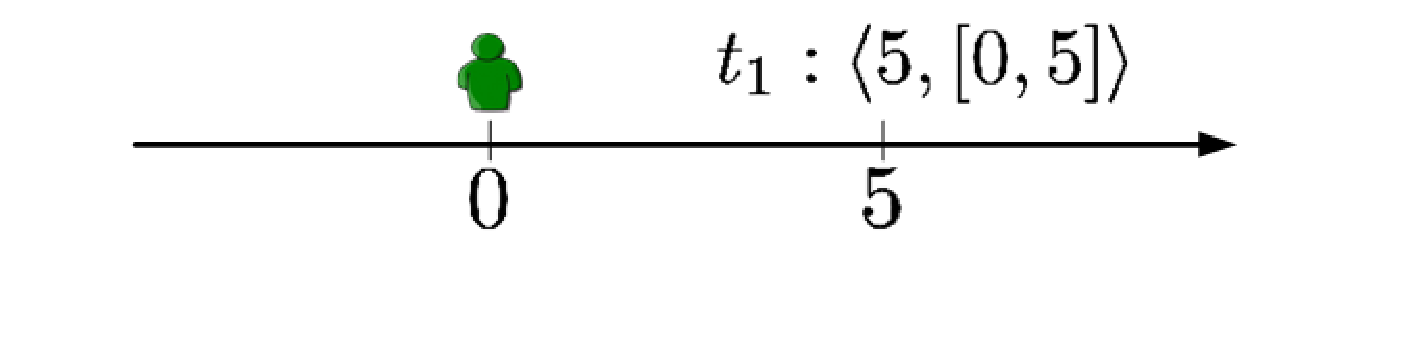
\includegraphics[width = 0.30\columnwidth]{figures/proof0}
    }
    \subfigure[$t = 2$, case $1$]{
        \label{fig:prooft21}
        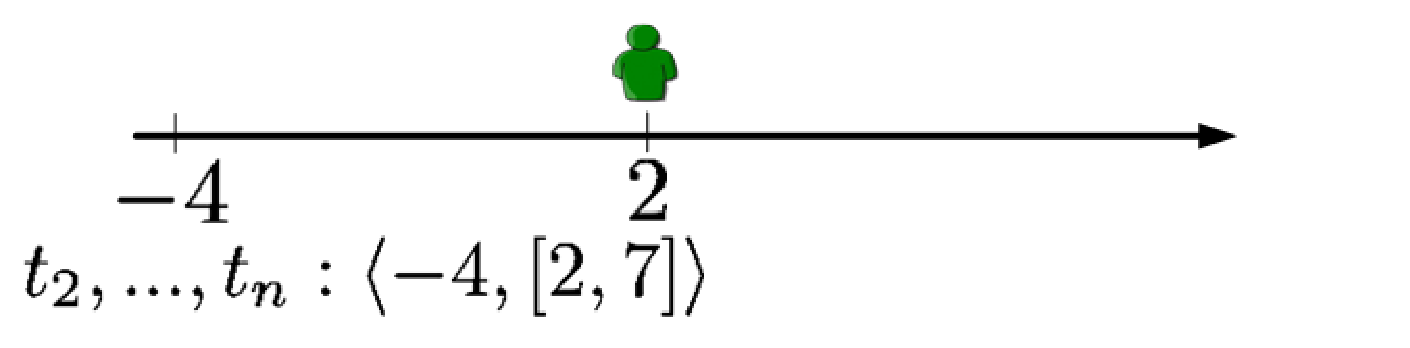
\includegraphics[width = 0.30\columnwidth]{figures/proof21}
    }
    \subfigure[$t = 2$, case $2$]{
        \label{fig:prooft22}
        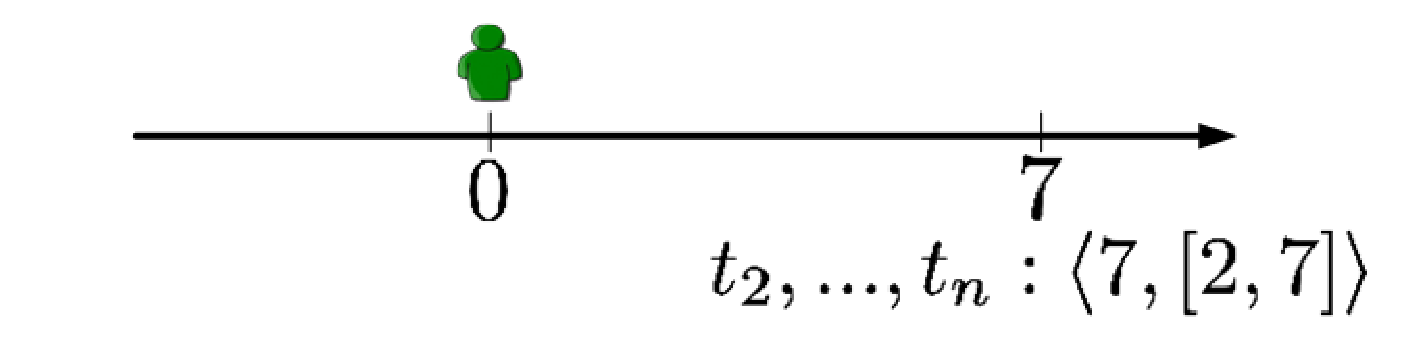
\includegraphics[width = 0.30\columnwidth]{figures/proof22}
    }
    \vspace{-0.15in}
    \caption{Adversary Generated Input}
    \label{fig:quality}
\end{figure}

\cref{th:comp_ratio} shows that for any deterministic online algorithm for OnlineTASC there exists a worst case scenario where the competitive ratio is very small and hence, there is no theoretical bound for the OnlineTASC problem. However, in the following sections we propose algorithms for OnlineTASC that generate close to optimal results when applied to both real-world and synthetic data.

%The equivalent decision problem for TASC is to decide if there exists a matching $M$ with value $K$ and is denoted as TASC$\left\langle W, T, d, K \right\rangle$. In this section we use a slightly modified version of the well known Hamiltonian Path Problem. We call it the Minimum Length Hamiltonian Path Problem (Min-Ham-Path) and define it as follows:

%\begin{definition}[Min-Ham-Path]
%Given a directed graph $G(V,E)$ where each edge $e \in E$ is assigned a length $l: E \rightarrow \mathbb{R}$, a source node $s$ and a length $L \in \mathbb{R}$, the Min-Ham-Path problem $\left\langle G, l, s, L \right\rangle$ is to decide whether there exists a path in $G$ that starts from $s$, visits every other node exactly once and has a length of at most $L$.
%\end{definition}

%\begin{theorem}
%\label{th:MinHam}
%The Min-Ham-Path problem is NP-Hard.
%\end{theorem}

%\begin{proof}
%Proof is shown in \cref{app:MinHamProof}.
%In order to prove the NP-Hardness of Min-Ham-Path we show Ham-Path $\leq_p$ Min-Ham-Path. The Hamiltonian Path problem asks the following question: Given a directed graph $G(V,E)$ does there exist a path that goes through every node exactly once?

%Given an instance of the Ham-Path problem $\left\langle G \right\rangle$ we modify graph $G(V,E)$ and generate a new graph $G'(V', E')$ where $V' = V \cup \left\{ o \right\}$ and $E' = E \cup \left\{ \left\langle o, v \right\rangle : v \in V \right\}$. Also, for every $e \in E'$ we Assume $l(e) = 1$.

%Now we show that Ham-Path$\left\langle G \right\rangle$ is true if and only if Min-Ham-Path$\left\langle G', l, o, n \right\rangle$ is true where $n$ is the number of vertices in $G$. If Min-Ham-Path returns a path of length $n$, we can remove the first edge from the path which results in a Hamiltonian Path for the Ham-Path$\left\langle G \right\rangle$ problem. On the other hand every Hamiltonian Path on graph $G$ has length $n-1$. By adding vertex $o$ and connecting it to the starting vertex, we end up with a Hamiltonian Path of length $n$ on $G'$.
%\end{proof}

%\begin{theorem}
%\label{th:TASC}
%The TASC problem is NP-Complete.
%\end{theorem}

%\begin{proof}
%Proof is shown in \cref{app:TASCProof}
%We start the proof by showing that the decision problem of TASC is \textit{verifiable} in polynomial time. Given a matching $M$, we can check that no task is assigned to more than one worker in polynomial time. Furthermore, based on the definition of a valid match, checking the validity of a matching $M$ can be done in polynomial time as well. Finally, we can find the value of $M$ by adding the value of every task in $M$.

%We show TASC is NP-Hard by proving the reduction Min-Ham-Path $\leq_p$ TASC. Given an instance of the Min-Ham-Path problem $\left\langle G(V,E), l, o, K \right\rangle$ we reduce it to an instance of the TASC$\left\langle W, T, l', n-1 \right\rangle$ problem such that $W = \left\{ o \right\}$, $T = V \setminus \left\{ o \right\}$. For every task $t$ we set $t.v = 1$, $t.r = 0$ and $t.d = K$. Also for every $e \in E, l'(e) = l(e)$. In addition for every $e' \in \left( W \times T \right) \cup \left( T \times T \right) $ where $e' \not\in E$ we set $l'(e') = \infty$.

%Finally we show the result of Min-Ham-Path$\left\langle G, l, o, K \right\rangle$ is true if TASC$\left\langle W, T, l', n-1 \right\rangle$ is true where $n$ is the number of vertices in $G$. Considering that $\left\vert T \right\vert = n - 1$ and $t.v = 1$ for every $t \in T$, if there exists a matching with size $n - 1$ it means every task has been assigned to the single worker. Also, since the deadline of every task is $K$ the worker visits every task no later than $K$. Therefore, the path that the worker traverses starts at $o$ and goes through every other vertex $v \in V \setminus \left\{ o \right\}$, where the length of the path is no more than $K$.
%\end{proof}